% !TEX program = xelatex
\documentclass[11pt,a4paper]{article}

\usepackage[margin=1.8cm]{geometry}
\usepackage{fontspec}
\usepackage{xcolor}
\usepackage{graphicx}
\usepackage{tikz}
\usepackage{enumitem}
\usetikzlibrary{calc}

\definecolor{ink}{HTML}{1A1A1A}
\definecolor{mute}{HTML}{5C5C5C}
\definecolor{line}{HTML}{E6E6E6}
\definecolor{paper}{HTML}{FAFAFA}

\setmainfont{TeX Gyre Pagella}
\setsansfont{Montserrat}

\newcommand{\chiikologo}{%
  
\includegraphics[height=1.35cm]{../../public/chiikologosophie.png}%
}

\newcommand{\docheader}[1]{%
  \noindent
  \begin{tikzpicture}
    \fill[paper] (0,0) rectangle (\textwidth,2.1);
    \node[anchor=west] at (0.2,1.05) {\chiikologo};
    \node[anchor=east, align=right, text=ink] at (\textwidth-0.2,1.35) {%
      {\sffamily\bfseries\large Sophie Gomez --- Propuestas}\\[2pt]
      {\sffamily\color{mute}\small #1}\\[1pt]
      {\sffamily\color{mute}\footnotesize Chiiko · Documento de selección}
    };
  \end{tikzpicture}
  \vspace{0.35cm}
  {\color{line}\hrule height 0.6pt}
  \vspace{0.55cm}
}

% Generic icon card
\newcommand{\iconcard}[3]{%
  % #1 title, #2 description, #3 tikz drawing commands (inside 2.2x2.2 area)
  \begin{tikzpicture}
    \draw[line, line width=0.7pt, fill=white] (0,0) rectangle (5.55,4.1);
    \fill[paper] (0.35,1.55) rectangle (5.2,3.7);
    \begin{scope}[shift={(2.775,2.62)}]
      #3
    \end{scope}
    \node[anchor=north west, font=\sffamily\bfseries\small, text=ink] at (0.3,1.35) {#1};
    \node[anchor=north west, font=\sffamily\scriptsize, text=mute, text width=4.9cm] at (0.3,0.95) {#2};
  \end{tikzpicture}%
}

\pagestyle{empty}
\setlength{\parindent}{0pt}

\begin{document}
\color{ink}

\docheader{02 · Iconos menú hamburguesa (3 líneas)}

{\sffamily
\textbf{Instrucciones para Sophie}\\[4pt]
{\color{mute}
Estas son propuestas visuales del icono de menú (las clásicas ``tres líneas'').
Todas se pueden implementar como SVG en el sitio. Elige 1 favorita
(y si quieres, una alternativa para el estado ``cerrar / X'').
}
}

\vspace{0.5cm}

\section*{{\sffamily Grupo A --- Clásicos}}

\noindent
\begin{tabular}{@{}p{0.5\textwidth-0.15cm}@{\hspace{0.3cm}}p{0.5\textwidth-0.15cm}@{}}
\iconcard{A1 · Equal bars}{Tres barras iguales, extremos cuadrados. El estándar más limpio.}{%
  \foreach \y in {-0.42,0,0.42} {
    \fill[ink] (-0.7,\y-0.055) rectangle (0.7,\y+0.055);
  }
}
&
\iconcard{A2 · Rounded caps}{Barras con puntas redondeadas. Más suave, menos técnico.}{%
  \foreach \y in {-0.42,0,0.42} {
    \draw[ink, line width=2.1pt, line cap=round] (-0.7,\y) -- (0.7,\y);
  }
}
\\[0.25cm]
\iconcard{A3 · Thin Swiss}{Líneas finas, mucho aire. Estética suiza / minimal.}{%
  \foreach \y in {-0.45,0,0.45} {
    \draw[ink, line width=1.1pt] (-0.75,\y) -- (0.75,\y);
  }
}
&
\iconcard{A4 · Bold editorial}{Barras más gruesas. Presencia fuerte en header oscuro o claro.}{%
  \foreach \y in {-0.4,0,0.4} {
    \fill[ink] (-0.72,\y-0.09) rectangle (0.72,\y+0.09);
  }
}
\end{tabular}

\vspace{0.35cm}
\section*{{\sffamily Grupo B --- Variaciones de longitud}}

\noindent
\begin{tabular}{@{}p{0.5\textwidth-0.15cm}@{\hspace{0.3cm}}p{0.5\textwidth-0.15cm}@{}}
\iconcard{B1 · Cascada corta}{Línea superior e inferior largas; media más corta. Dinámico.}{%
  \draw[ink, line width=2pt, line cap=round] (-0.7,0.42) -- (0.7,0.42);
  \draw[ink, line width=2pt, line cap=round] (-0.7,0) -- (0.25,0);
  \draw[ink, line width=2pt, line cap=round] (-0.7,-0.42) -- (0.7,-0.42);
}
&
\iconcard{B2 · Escalera derecha}{Las tres líneas decrecen a la derecha. Toque fashion.}{%
  \draw[ink, line width=2pt, line cap=round] (-0.7,0.42) -- (0.7,0.42);
  \draw[ink, line width=2pt, line cap=round] (-0.7,0) -- (0.35,0);
  \draw[ink, line width=2pt, line cap=round] (-0.7,-0.42) -- (0.0,-0.42);
}
\\[0.25cm]
\iconcard{B3 · Solo media corta}{Clásico con detalle sutil: solo la barra central más corta.}{%
  \draw[ink, line width=2pt, line cap=round] (-0.7,0.42) -- (0.7,0.42);
  \draw[ink, line width=2pt, line cap=round] (-0.45,0) -- (0.45,0);
  \draw[ink, line width=2pt, line cap=round] (-0.7,-0.42) -- (0.7,-0.42);
}
&
\iconcard{B4 · Alineado a la derecha}{Barras ancladas a la derecha (encaja con menú a la derecha).}{%
  \draw[ink, line width=2pt, line cap=round] (-0.2,0.42) -- (0.7,0.42);
  \draw[ink, line width=2pt, line cap=round] (-0.45,0) -- (0.7,0);
  \draw[ink, line width=2pt, line cap=round] (-0.7,-0.42) -- (0.7,-0.42);
}
\end{tabular}

\newpage
\docheader{02 · Iconos menú (cont.)}

\section*{{\sffamily Grupo C --- Con marco / botón}}

\noindent
\begin{tabular}{@{}p{0.5\textwidth-0.15cm}@{\hspace{0.3cm}}p{0.5\textwidth-0.15cm}@{}}
\iconcard{C1 · Círculo outline}{Icono dentro de círculo. Más ``botón'', menos texto.}{%
  \draw[ink, line width=1.2pt] (0,0) circle (0.95);
  \foreach \y in {-0.32,0,0.32} {
    \draw[ink, line width=1.6pt, line cap=round] (-0.42,\y) -- (0.42,\y);
  }
}
&
\iconcard{C2 · Cuadrado outline}{Marco cuadrado fino. Look editorial / press.}{%
  \draw[ink, line width=1.1pt] (-0.95,-0.95) rectangle (0.95,0.95);
  \foreach \y in {-0.32,0,0.32} {
    \draw[ink, line width=1.6pt, line cap=round] (-0.45,\y) -- (0.45,\y);
  }
}
\\[0.25cm]
\iconcard{C3 · Pill / pastilla}{Contenedor redondeado. Moderno, amable.}{%
  \draw[ink, line width=1.2pt, rounded corners=0.55cm] (-1.05,-0.7) rectangle (1.05,0.7);
  \foreach \y in {-0.28,0,0.28} {
    \draw[ink, line width=1.6pt, line cap=round] (-0.45,\y) -- (0.45,\y);
  }
}
&
\iconcard{C4 · Disco sólido}{Círculo relleno + líneas claras. Alto contraste.}{%
  \fill[ink] (0,0) circle (0.95);
  \foreach \y in {-0.3,0,0.3} {
    \draw[white, line width=1.7pt, line cap=round] (-0.4,\y) -- (0.4,\y);
  }
}
\end{tabular}

\vspace{0.35cm}
\section*{{\sffamily Grupo D --- Con etiqueta de texto}}

\noindent
\begin{tabular}{@{}p{0.5\textwidth-0.15cm}@{\hspace{0.3cm}}p{0.5\textwidth-0.15cm}@{}}
\iconcard{D1 · MENU + barras}{Texto MENU a la izquierda de las líneas. Muy portfolio.}{%
  \node[font=\sffamily\bfseries\fontsize{7}{8}\selectfont, text=ink, anchor=east] at (-0.15,0) {MENU};
  \foreach \y in {-0.28,0,0.28} {
    \draw[ink, line width=1.5pt, line cap=round] (0.05,\y) -- (0.85,\y);
  }
}
&
\iconcard{D2 · Barras + MENU}{Líneas primero, texto después. Equilibrado.}{%
  \foreach \y in {-0.28,0,0.28} {
    \draw[ink, line width=1.5pt, line cap=round] (-0.85,\y) -- (-0.05,\y);
  }
  \node[font=\sffamily\bfseries\fontsize{7}{8}\selectfont, text=ink, anchor=west] at (0.15,0) {MENU};
}
\\[0.25cm]
\iconcard{D3 · [ Menu ]}{Estilo actual del sitio: tipográfico con corchetes.}{%
  \node[font=\sffamily\fontsize{9}{11}\selectfont, text=ink] {[\thinspace Menu\thinspace]};
}
&
\iconcard{D4 · Menu · · ·}{Palabra + tres puntos verticales sutiles (variante).}{%
  \node[font=\sffamily\bfseries\fontsize{8}{9}\selectfont, text=ink, anchor=east] at (0.05,0) {Menu};
  \foreach \y in {-0.28,0,0.28} {
    \fill[ink] (0.35,\y) circle (0.045);
  }
}
\end{tabular}

\newpage
\docheader{02 · Iconos menú (cont.)}

\section*{{\sffamily Grupo E --- Estado abierto (cerrar)}}

{\sffamily\color{mute}\small
Además del icono cerrado, conviene elegir cómo se ve el botón cuando el menú está abierto.
}

\vspace{0.35cm}
\noindent
\begin{tabular}{@{}p{0.5\textwidth-0.15cm}@{\hspace{0.3cm}}p{0.5\textwidth-0.15cm}@{}}
\iconcard{E1 · X clásica}{Dos líneas cruzadas. El cierre más universal.}{%
  \draw[ink, line width=2pt, line cap=round] (-0.55,-0.55) -- (0.55,0.55);
  \draw[ink, line width=2pt, line cap=round] (-0.55,0.55) -- (0.55,-0.55);
}
&
\iconcard{E2 · X fina}{Misma idea, trazo delgado. Más editorial.}{%
  \draw[ink, line width=1.2pt, line cap=round] (-0.55,-0.55) -- (0.55,0.55);
  \draw[ink, line width=1.2pt, line cap=round] (-0.55,0.55) -- (0.55,-0.55);
}
\\[0.25cm]
\iconcard{E3 · CLOSE tipográfico}{Sin icono: solo la palabra Close / Fermer / Cerrar.}{%
  \node[font=\sffamily\bfseries\fontsize{8}{9}\selectfont, text=ink] {CLOSE};
}
&
\iconcard{E4 · Barras $\rightarrow$ X animable}{Parte del mismo SVG: las 3 barras rotan a X.}{%
  \draw[ink, line width=2pt, line cap=round, rotate=45] (-0.6,0) -- (0.6,0);
  \draw[ink, line width=2pt, line cap=round, rotate=-45] (-0.6,0) -- (0.6,0);
  \node[font=\sffamily\fontsize{5}{6}\selectfont, text=mute] at (0,-0.85) {animable};
}
\end{tabular}

\vspace{0.55cm}
\section*{{\sffamily Combinaciones recomendadas}}

{\sffamily\small
\begin{itemize}[leftmargin=1.1em, itemsep=0.2em]
  \item \textbf{Look actual del sitio:} D3 \texttt{[ Menu ]} + E3 tipográfico (ya implementado).
  \item \textbf{Minimal puro:} A3 Thin Swiss + E2 X fina.
  \item \textbf{Fashion:} B2 Escalera derecha + E1 X clásica.
  \item \textbf{Botón claro:} C1 Círculo outline + E1.
  \item \textbf{Alto contraste:} C4 Disco sólido + E1 en negativo.
\end{itemize}
}

\vspace{0.45cm}
\noindent
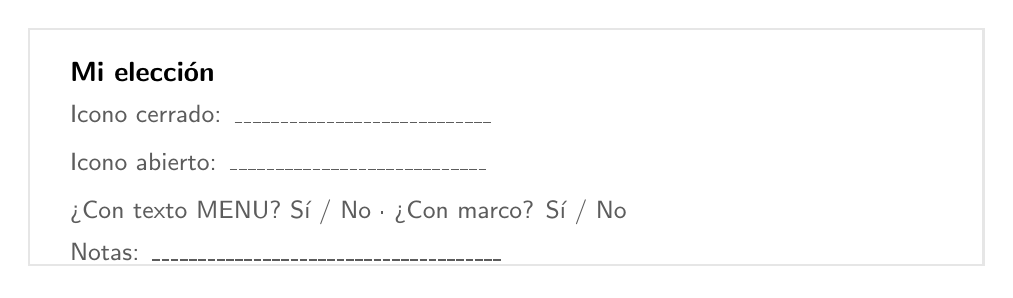
\begin{tikzpicture}
  \draw[line, line width=0.8pt] (0,0) rectangle (\textwidth,3.0);
  \node[anchor=north west, font=\sffamily\bfseries] at (0.4,2.7) {Mi elección};
  \node[anchor=north west, font=\sffamily\small, text=mute] at (0.4,2.15) {Icono cerrado: \_\_\_\_\_\_\_\_\_\_\_\_\_\_\_\_\_\_\_\_\_\_\_\_\_\_\_\_};
  \node[anchor=north west, font=\sffamily\small, text=mute] at (0.4,1.55) {Icono abierto: \_\_\_\_\_\_\_\_\_\_\_\_\_\_\_\_\_\_\_\_\_\_\_\_\_\_\_\_};
  \node[anchor=north west, font=\sffamily\small, text=mute] at (0.4,0.95) {¿Con texto MENU?  Sí / No   ·   ¿Con marco?  Sí / No};
  \node[anchor=north west, font=\sffamily\small, text=mute] at (0.4,0.4) {Notas: \_\_\_\_\_\_\_\_\_\_\_\_\_\_\_\_\_\_\_\_\_\_\_\_\_\_\_\_\_\_\_\_\_\_\_\_\_\_};
\end{tikzpicture}

\vspace{0.7cm}
{\sffamily\color{mute}\footnotesize
Chiiko · Propuestas de icono de menú para Sophie Gomez · Los dibujos se exportan como SVG en implementación
}

\end{document}
